\documentclass[]{beamer}
\usepackage[utf8]{inputenc}
\usepackage[T1]{fontenc}
\usepackage[portuges,brazilian]{babel}
\usepackage{graphicx}
\usepackage[sfdefault]{quattrocento}
\usepackage{multicol}
\usepackage{hyperref}
\usepackage[alf]{abntex2cite}
\usepackage{color}
\usepackage{tabularx}
\useoutertheme{infolines}
\useinnertheme{rectangles}
\usefonttheme{professionalfonts}
\title{Módulo de pré visualização para a ferramenta CGT}
\subtitle{Ceará Game Tools}
\author[Joel]{Joel Rocha}
\institute[IFCE]{Orientador: Prof. Dr. Carlos Hairon
   \par Engenharia de Computação
   \par Instituto Federal de Educação, Ciência e Tecnologia do Ceará}
\date{Dezembro, 2015}
\logo{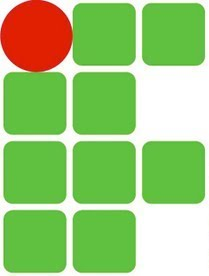
\includegraphics[width=0.8cm]{images/logo.jpg}}

\begin{document}
   \begin{frame}
      \titlepage
   \end{frame}

   \begin{frame}{\contentsname}
      \tableofcontents[hideallsubsections]
   \end{frame}

   \section{Introdução}
   \subsection{Indústria de jogos digitais}
   \begin{frame}
      \frametitle{Qual a importância dos jogos?}
      \framesubtitle{Introdução}
      \begin{itemize}
         \item Geração de emprego e renda {\scriptsize (produtor, desenvolvedor, testador, \emph{designer}, roteirista, dublador)}.
         \item Inovação tecnológica.
         \item Diversidade no público alvo.
         \item Várias plataformas (PC, Console, Mobile).
         \item Movimenta em torno de US\$ 82 bilhões. \cite{ind-bra-relatorio}
      \end{itemize}
   \end{frame}
   \begin{frame}
      \begin{center}
         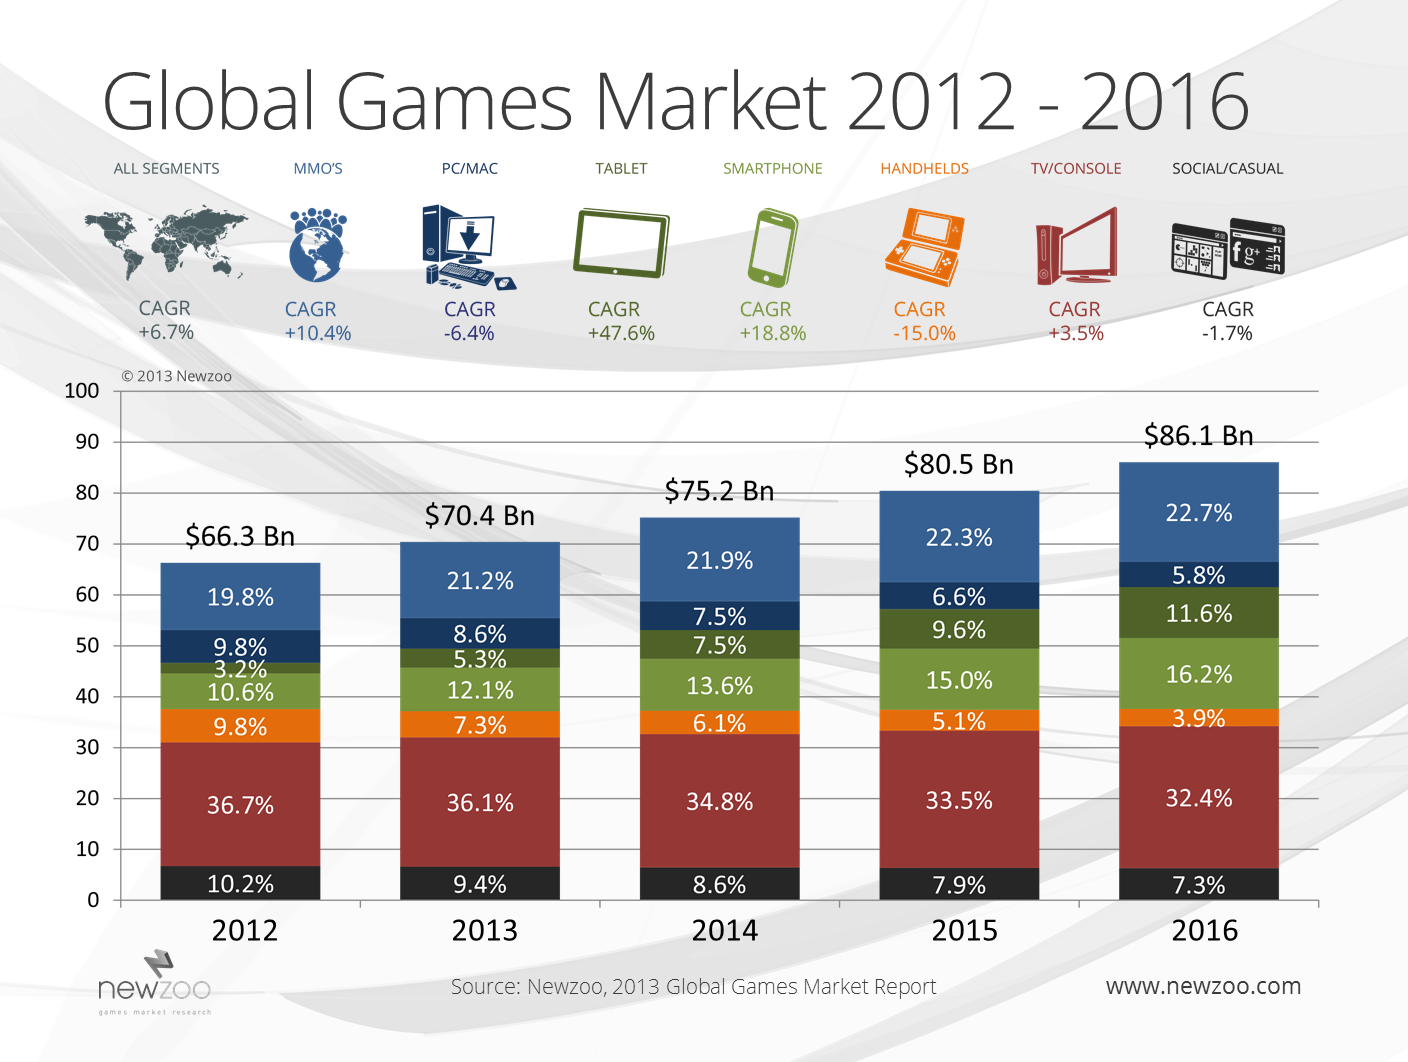
\includegraphics[width=\textwidth]{images/Newzoo_Global_Games_Market_2012-2016_V1.png}
      \end{center}
   \end{frame}
   \subsection{Projeto CGT}
   \begin{frame}
      \frametitle{O que é o Projeto CGT?}
      \framesubtitle{Introdução}
      Projeto Ceará \emph{Games Tools} tem o objetivo de oferecer uma ferramenta para a construção de jogos onde qualquer um poderá criar seu próprio jogo. \cite{website:projeto-cgt}
   \end{frame}
   \subsection{Vínculo CNPQ}
   \begin{frame}
      \frametitle{Projeto CGT e o CNPQ}
      \framesubtitle{Introdução}
      \begin{itemize}
         \item Pesquisa, Desenvolvimento e Comercialização de Games Temáticos da Cultura Cearense.
         \item \emph{Software livre}.
         \item Multiplataforma.
         \item Edital 80 de 2013, processo 409227/2013-7.
      \end{itemize}
   \end{frame}
   \subsection{Projeto de extensão}
   \begin{frame}
      \begin{columns}[T]
         \begin{column}{0.48\textwidth}
            \frametitle{Projeto de extensão}
            \framesubtitle{Introdução}
            \begin{itemize}
               \item Curso de desenvolvimento de jogos digitais;
               \item Para 14 jovens do ensino fundamental e médio;
               \item Difundir a cultura do desenvolvimento de jogos;
               \item Ferramentas de desenvolvimento:
                  \begin{itemize}
                     \item Construct 2 e
                     \item Ferramenta CGT (versão 2.0).
                  \end{itemize}
            \end{itemize}
         \end{column}
         \begin{column}{0.48\textwidth}
            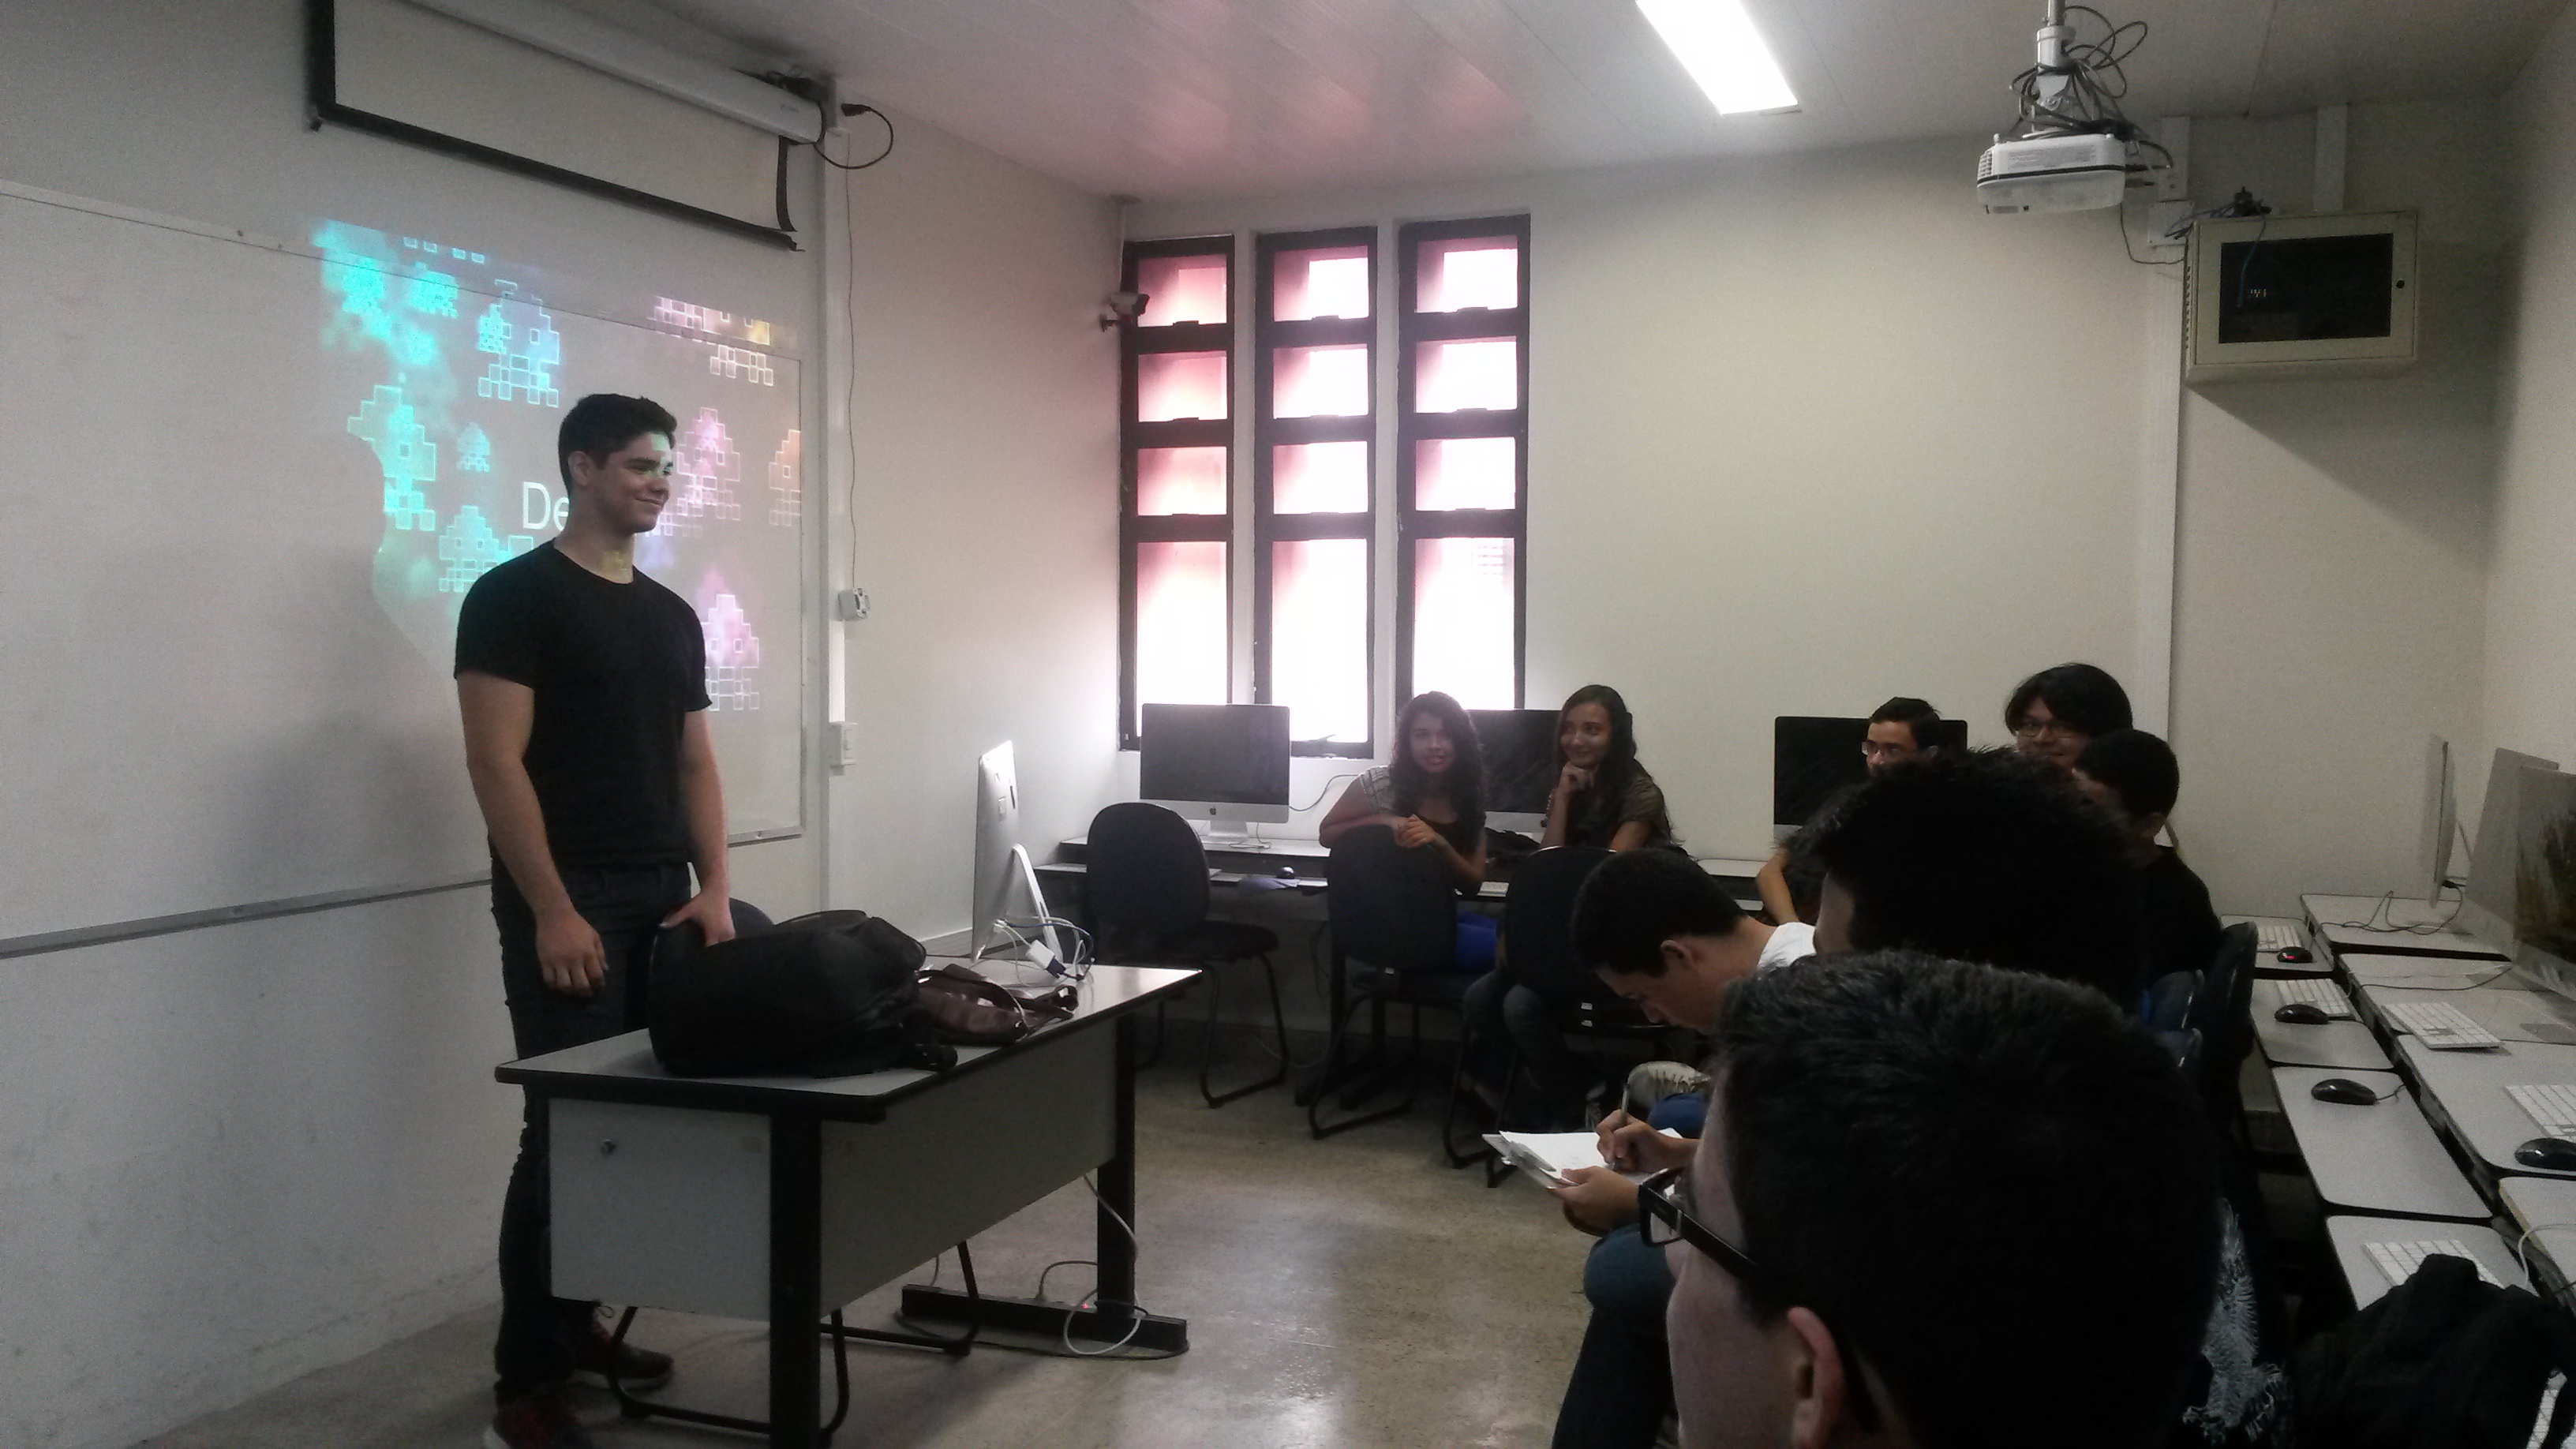
\includegraphics[width=\textwidth]{images/ext/20150921_101616.jpg}
         \end{column}
      \end{columns}
   \end{frame}

   \begin{frame}
      \frametitle{Retorno dos usuários}
      \framesubtitle{Introdução}
      \begin{columns}[T]
         \begin{column}{0.48\textwidth}
            \begin{itemize}
               \item Fácil aprendizagem;
               \item Correção de erros;
               \item 93\% dos usuários preferem a ferramenta CGT;
               \item Motivos:
                  \begin{itemize}
                     \item Idioma;
                     \item Simplicidade e
                     \item Recursos disponíveis.
                  \end{itemize}
            \end{itemize}
         \end{column}
         \begin{column}{0.48\textwidth}
            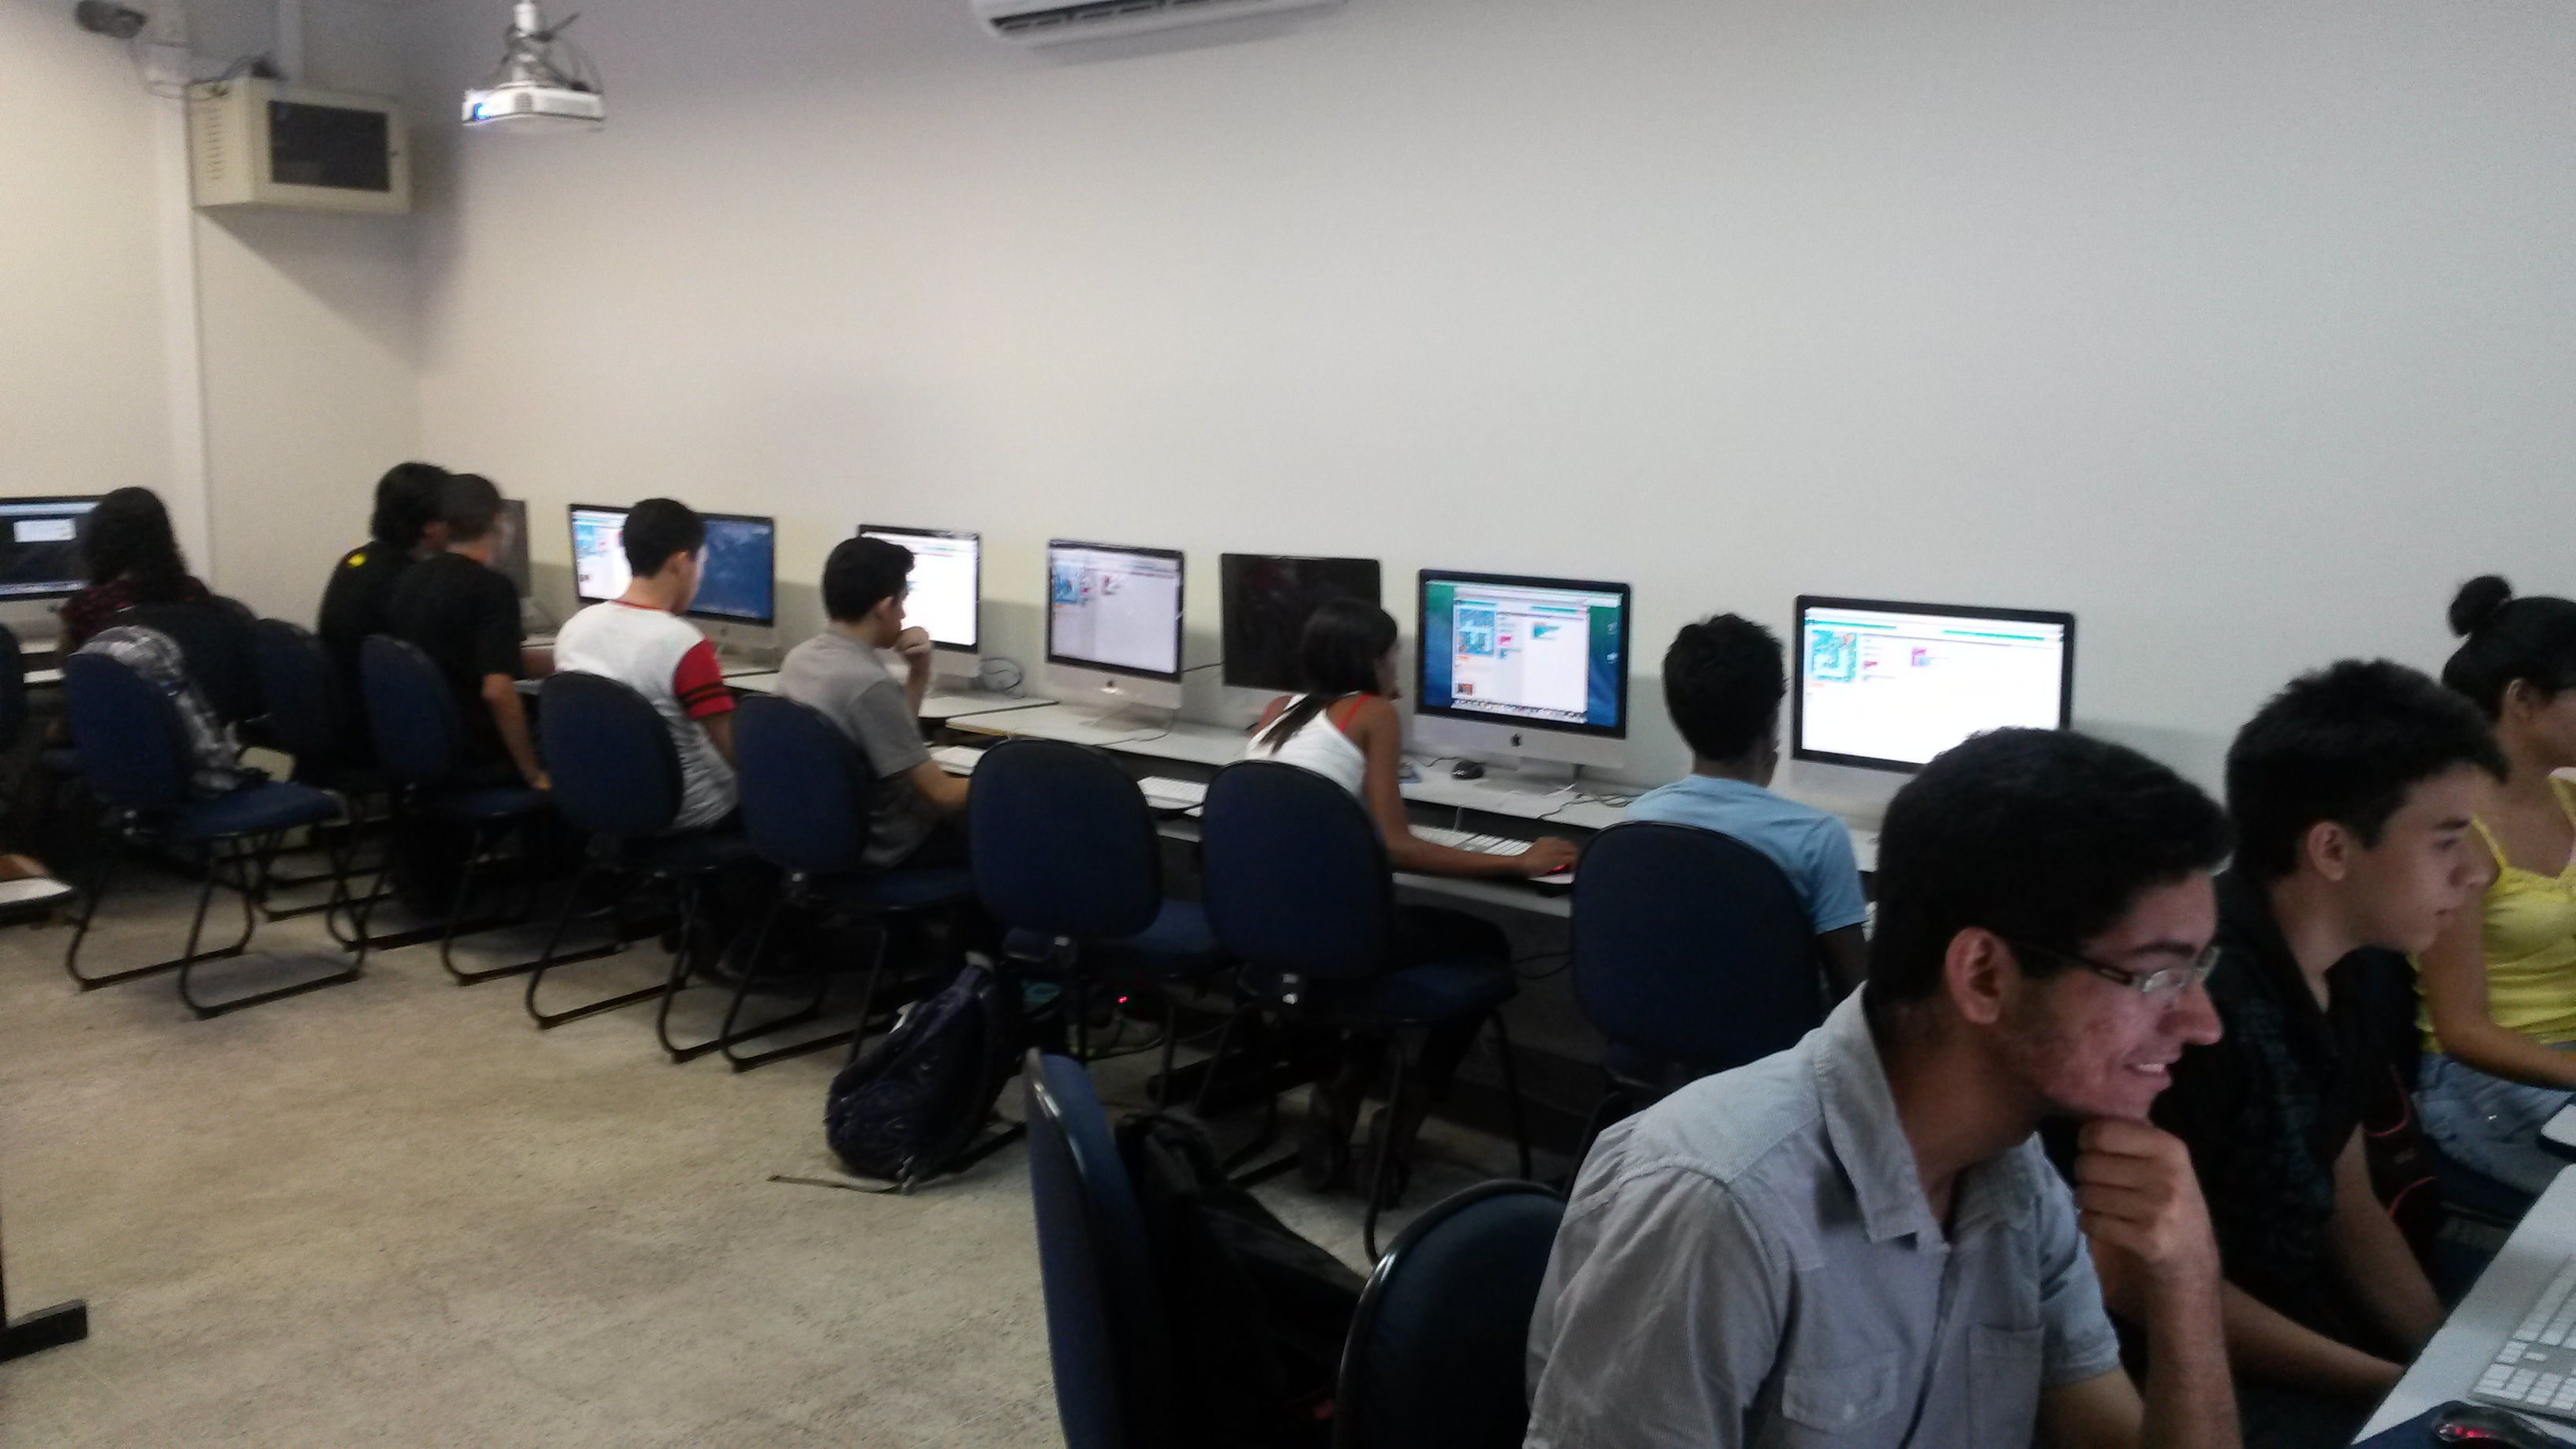
\includegraphics[width=\textwidth]{images/ext/20150902_110944.jpg}
         \end{column}
      \end{columns}
   \end{frame}

   \subsection{Introdução ao problema}
   \begin{frame}
      \frametitle{Problemas da ferramenta 1.0}
      \framesubtitle{Introdução}
      \begin{itemize}
         \item Controles confusos;
         \item Ausência de \emph{feedback};
         \item \textbf{Pré visualização.}
      \end{itemize}
   \end{frame}
   \begin{frame}
      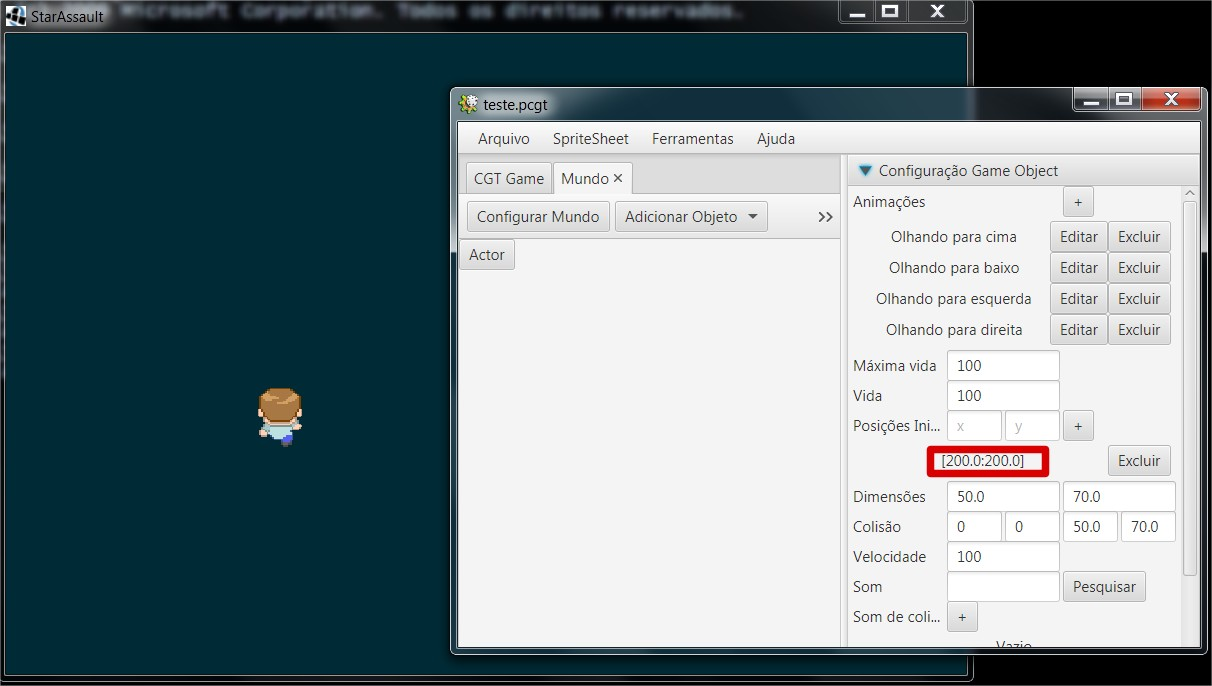
\includegraphics[width=\textwidth]{images/problema-1.jpg}
   \end{frame}

   \begin{frame}
      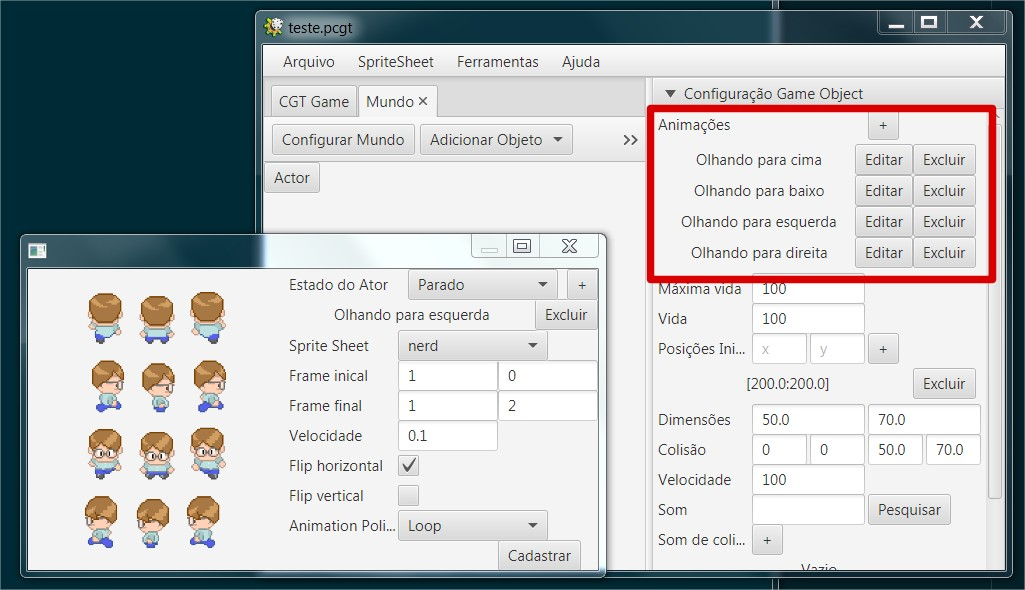
\includegraphics[width=\textwidth]{images/problema-2.jpg}
   \end{frame}

   \section{Descrição das melhorias}
   \subsection{Problema I - Organização dos objetos}
   \subsubsection{Descrição}
   \begin{frame}
      \frametitle{Organização dos objetos do jogo}
      \framesubtitle{Descrição do problema}
      \begin{itemize}
         \item Jogos possuem muitos objetos e são longos.
         \item Hierarquia entre objetos.
         \item As características importam na organização.
         \item Tipos de objetos:
            \begin{multicols}{2}
               \begin{itemize}
                  \item Mundo,
                  \item Ator,
                  \item Inimigo,
                  \item Opositor,
                  \item Bônus,
                  \item Projétil,
                  \item Tela,
                  \item Botão de tela,
                  \item Barra de vida e
                  \item Barra de munição.
               \end{itemize}
            \end{multicols}
      \end{itemize}
   \end{frame}

   \begin{frame}
      \begin{center}
         \begin{tabular}{ p{6em} | p{20em} }
         \textbf{Objeto} & \textbf{Descrição} \\
         \hline
         Mundo & Fase do jogo definindo o plano de fundo.  \\
         \hline
         Ator & Objeto controlado pelo jogador. \\
         \hline
         Inimigo & Objeto que causa dano ao ator e impede os objetivos dele. \\
         \hline
         Opositor & Objeto que impede ações do ator.  \\
         \hline
         Bônus & Objeto que promove bônus ao ator. \\
         \hline
         Projétil & Objeto que pode ser arremessado pelo ator. \\
         \hline
         Tela & Representa uma tela do jogo. \\
         \hline
         Botão de tela & Botão de uma tela do jogo. \\
         \hline
         Vida de um objeto & Mostra a quantidade de vida que um objeto possui. \\
         \hline
         Munição de um objeto & A quantidade de projéteis que o ator ainda pode arremessar. \\
      \end{tabular}
   \end{center}
   \end{frame}

   \begin{frame}
      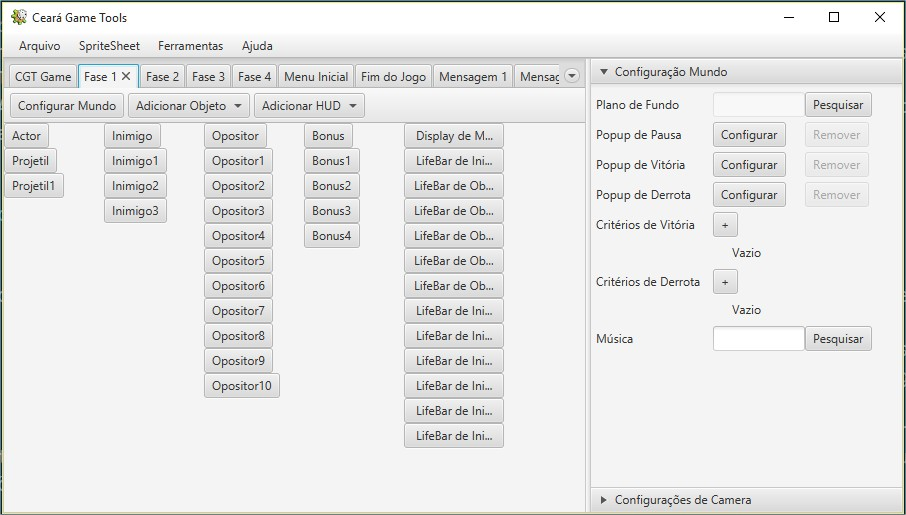
\includegraphics[width=\textwidth]{images/objetos_disposicao.jpg}
   \end{frame}

   \subsubsection{Resolução}
   \begin{frame}
      \frametitle{Organização de objetos no jogo}
      \framesubtitle{Resolução do problema}

      \begin{columns}[T]
         \begin{column}{0.48\textwidth}
            \begin{itemize}
               \item Árvore de objetos;
               \item Visão de tudo que existe no jogo;
               \item Objetos acessíveis a poucos cliques;
               \item Ocupa menor espaço na janela.
            \end{itemize}
         \end{column}
         \begin{column}{0.48\textwidth}
            \begin{center}
            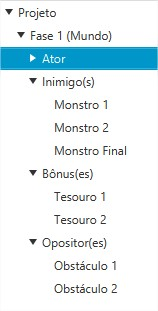
\includegraphics[width=0.48\textwidth]{images/arvore_objetos.jpg}
            \end{center}
         \end{column}
      \end{columns}
   \end{frame}

   \begin{frame}
      \begin{center}
         \begin{tabular}{| p{8cm} | l | }
            \hline
            \textbf{Item} & \textbf{Item superior} \\
            \hline
            Projeto & (Raiz) \\
            Mundo & Projeto \\
            Ator, Inimigos, Bônus(es), Opositor(es) & Mundo \\
            Projetil & Ator \\
            Barra de vida & Ator, Inimigo \\
            Munição & Projétil \\
            Tela & Projeto \\
            Botão de tela & Tela \\
            \hline
         \end{tabular}
      \end{center}
   \end{frame}

   \subsection{Problema II - Painéis de configuração}
   \subsubsection{Descrição}
   \begin{frame}
      \frametitle{Painéis de configuração}
      \framesubtitle{Problemas encontrados}
      \begin{itemize}
         \item Falta clareza;
         \item Valores possíveis (mínimo e máximo);
         \item Fluidez da aplicação;
         \item Mostrar o significado de cada propriedade ao usuário.
      \end{itemize}
   \end{frame}

   \begin{frame}
      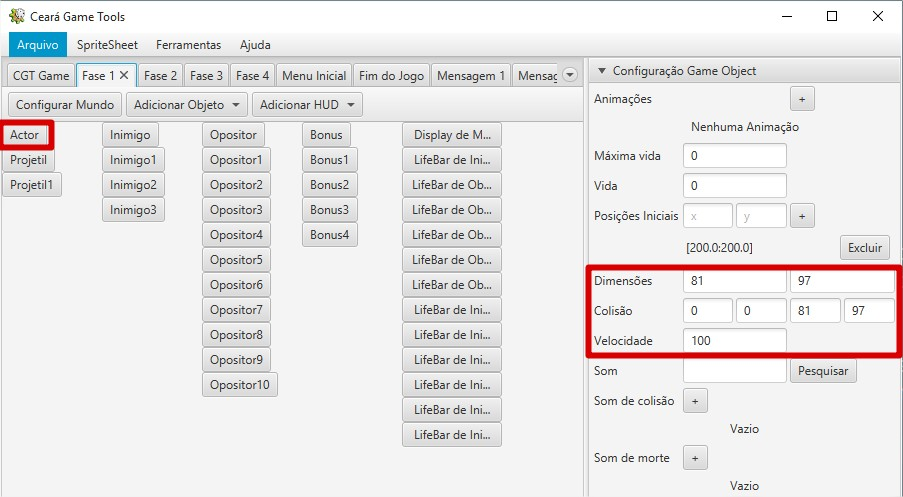
\includegraphics[width=\textwidth]{images/obj_dimensoes.jpg}
   \end{frame}

   \subsubsection{Resolução}
   \begin{frame}
      \frametitle{Painéis de configuração}
      \framesubtitle{Resolução do problema}

      \begin{itemize}
         \item Evitar diálogos (janelas que sobrepõem a janela principal);
         \item Interagir com demais áreas;
         \item Aprimorar os painéis da \texttt{ferramenta 1.0} para a \texttt{ferramenta 2.0} (exemplo configuração das animações de um objeto).
         \item Segregar as configurações dos objetos.
      \end{itemize}
   \end{frame}

   \begin{frame}
      \begin{center}
         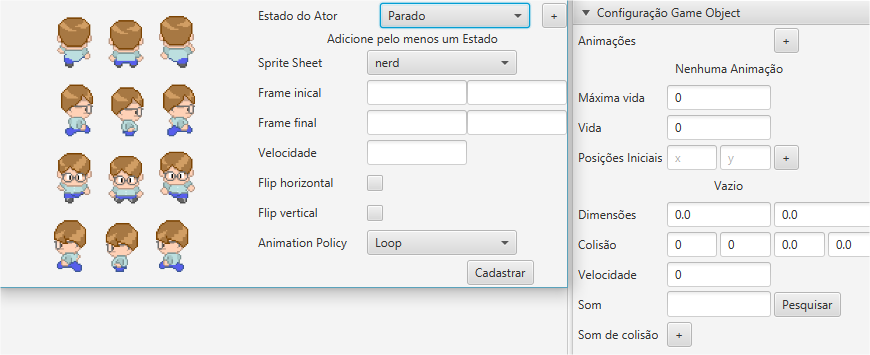
\includegraphics[width=\textwidth]{images/add_animacao_1.png}
      \end{center}
   \end{frame}

   \begin{frame}
      \begin{center}
         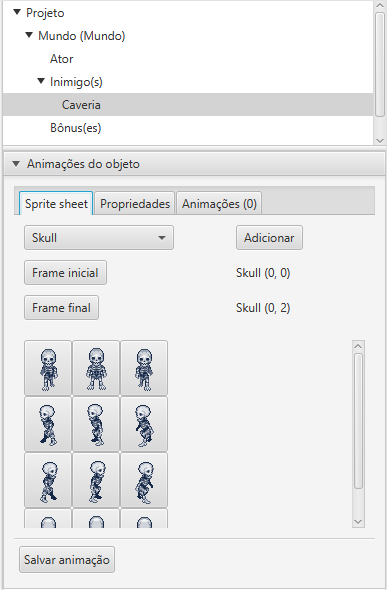
\includegraphics[width=0.4\textwidth]{images/add_animacao_2.png}
      \end{center}
   \end{frame}

   \subsection{Problema III - Ausência de pré visualização dos objetos}
   \subsubsection{Descrição}
   \begin{frame}
      \frametitle{Pré visualização}
      \framesubtitle{Problemas encontrados}
         \begin{itemize}
            \item Executar o jogo com muita frequência;
            \item Entender melhor as configurações feitas;
            \item A prévia contribui para problemas anteriores;
         \end{itemize}
   \end{frame}

   \begin{frame}
      \begin{center}
         \begin{tabular}{p{12em} | p{12em}}
            \textbf{Objeto(s)} & \textbf{Atributo(s)} \\
            \hline
            Mundo e tela do jogo & Plano de fundo \\
            \hline
            Ator, inimigo, bônus, opositor e projétil & Animações (\emph{spritesheet}), posição inicial, dimensões e área de colisão. \\
            \hline
            Botão de uma tela & Posição, dimensões, textura do botão normal e textura quando for pressionado.\\
            \hline
            Munição do projétil & Posição, dimensões e ícone. \\
            \hline
            Barra de vida de um objeto & Posição, dimensões, textura do preenchimento da barra e textura do plano de fundo. \\
         \end{tabular}
      \end{center}
   \end{frame}

   \subsubsection{Resolução}
   \begin{frame}
      \frametitle{Resolução do problema}
      \framesubtitle{Pré visualização}

      \begin{block}{Área de pré visualização}
         Espaço na ferramenta responsável por mostrar os objetos que foram criados, possibilitando que sejam visualizados pelo usuário.
      \end{block}

      \begin{block}{Objetos nessa área devem}
         \begin{itemize}
            \item Refletir com as configurações feitas,
            \item Estar sincronizado com os itens da árvore e
            \item Ser fiéis ao jogo.
         \end{itemize}
      \end{block}

   \end{frame}

   \begin{frame}
      \begin{center}
         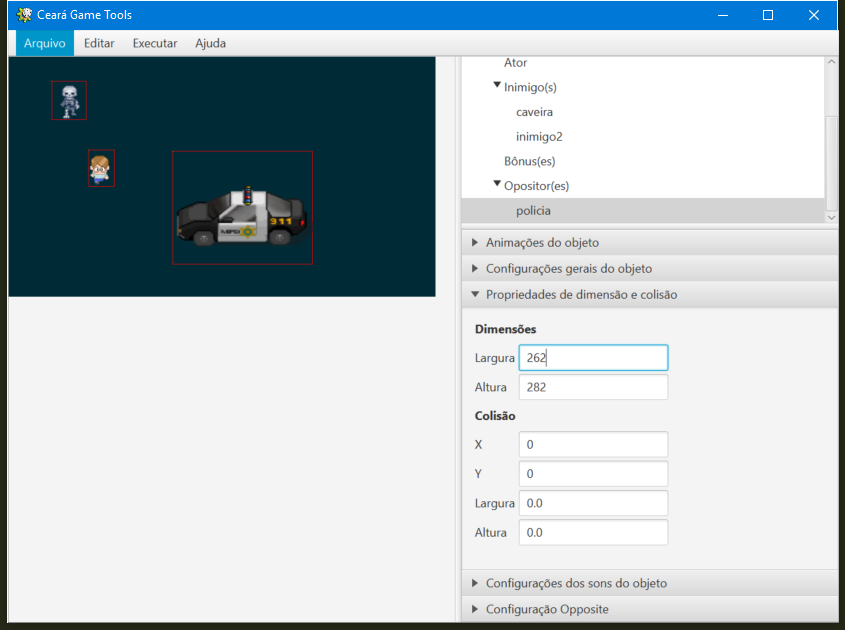
\includegraphics[width=0.9\textwidth]{images/preview2.png}
      \end{center}
   \end{frame}

   \section{Estudo de caso}
   \subsection{Análise}
   \begin{frame}
      \frametitle{Resultado das melhorias}
      \framesubtitle{Estudo de caso}

      \begin{itemize}
         \item Houve ganho? De quanto?
         \item As melhorias são percebidas pelo usuário?
         \item A pré visualização tornou a ferramenta mais efetiva?
      \end{itemize}
   \end{frame}

   \subsection{Método Keystroke-Level Model}
   \begin{frame}
      \frametitle{\emph{Keystroke-Level Model} (KLM)}
      \framesubtitle{Comparando as ferramentas}

      \begin{itemize}
         \item Método que atribui a todas as ações do usuário um intervalo de tempo;
         \item Usado para calcular a possível duração de uma tarefa;
         \item Dividi uma tarefa em várias sub tarefas passo-a-passo para quantificar o total;
         \item Fonte: \cite{klm-def}
      \end{itemize}
   \end{frame}

   \begin{frame}
      \begin{center}
         \begin{tabular}{| l | p{18em} | r |}
            \hline
            \textbf{Operação} & \textbf{Descrição} & \textbf{Tempo (s)} \\
            \hline
            K & Digitar uma tecla, é usado para quando o usuário digita qualquer tecla seja a letra \texttt{a} ou a tecla \texttt{SHIFT}.  & 0,12 \\
            P & Posicionar o ponteiro do mouse em algum local da tela.  & 1,1  \\
            B & Pressionar ou liberar os botões do mouse & 0,1 \\
            BB & Clique do mouse & 0,2 \\
            H & Mover a mão do teclado para o mouse. & 0,4 \\
            M & Pensar ou perceber algo relacionado ao sistema. & 1,2 \\
            \hline
         \end{tabular}
      \end{center}
   \end{frame}

   \subsection{Tarefas analisadas}
   \begin{frame}
      \frametitle{Tarefas analisadas}
      \framesubtitle{Estudo de caso}

      \begin{itemize}
         \item Selecionar um objeto já criado na ferramenta;
         \item Configurar os objetos de um mundo;
            \begin{itemize}
               \item Atribuir as dimensões;
               \item Posicionar o objeto;
               \item Criar animações;
            \end{itemize}
         \item Configurar uma tela;
            \begin{itemize}
               \item Selecionar plano de fundo;
               \item Criar um botão;
            \end{itemize}
      \end{itemize}
   \end{frame}

   \begin{frame}
      \frametitle{Selecionar um objeto}
      \framesubtitle{Exemplo de tarefa}
      {\small
      \begin{tabularx}{\textwidth}{X  X}
         \textbf{Primeira versão:}
         \begin{enumerate}
            \item Achar aba do objeto (M);
            \item Posicionar ponteiro na aba (P);
            \item Clicar na aba (BB);
            \item Achar o botão do objeto (M);
            \item Posicionar ponteiro no botão do objeto (P);
            \item Clicar no botão do objeto (BB);
         \end{enumerate}
         &
         \textbf{Nova versão:}
         \begin{enumerate}
            \item Achar objeto na árvore (M);
            \item Posicionar ponteiro no item (P);
            \item Clicar no item do objeto (BB);
         \end{enumerate}
         \\
         \texttt{M + 2BB + 2P = 2,4 + 0,4 + 2,2 =} \textbf{5,0s}
         &
         \texttt{M + BB + P = 1,2 + 0,2 + 1,1 =} \textbf{2,5s}
         \\
      \end{tabularx}}
   \end{frame}

   \subsection{Resultado da comparação}
   \begin{frame}
      \frametitle{Tabela de resultados}
      \framesubtitle{Estudo de caso}
      \begin{center}
            \begin{tabular}{ m{16em} | r | r }
               Configurar um objeto (7 animações)      & 3min 38s & \textcolor{green}{2min 39s} \\
               \hspace{2em}Configurar as dimensões     & 5,0s     & \textcolor{green}{2,5s} \\
               \hspace{2em}Configurar a posição        & 7,54s    & 7,54s \\
               \hspace{2em}Configurar uma animação     & 28,90s   & \textcolor{green}{20,96s} \\
               Configurar uma tela (com 2 botões)      & 46,3s    & \textcolor{green}{39,9s} \\
               \hspace{2em}Configurar textura          & 5,3s     & 5,3s \\
               \hspace{2em}Criar botão                 & 20,5s    & \textcolor{green}{17,3s} \\
               \hspace{4em}Configurar textura          & 11,5s    & 11,5s \\
               \hspace{4em}Posicionar botão            & 4,5s     & \textcolor{green}{1,3s} \\
               \hspace{4em}Configurar tamanho          & 4,5s     & 4,5s \\
               Selecionar um objeto                    & 5,0s     & \textcolor{green}{2,5s} \\
               \hline
               \textbf{Jogo com 20 objetos e 10 telas} & \textbf{1h 17min} & \textbf{\textcolor{green}{57min}} \\
         \end{tabular}
      \end{center}
   \end{frame}

   \section{Conclusão e trabalhos futuros}
   \begin{frame}
      \frametitle{Considerações finais}
      \framesubtitle{Conclusão}
      \begin{itemize}
         \item É possível tornar a ferramenta mais fácil, lógica e produtiva.
         \item Criar jogos de forma rápida.
         \item Sem conhecimento técnico.
         \item Baixo custo.
      \end{itemize}
   \end{frame}
   \begin{frame}
      \frametitle{Trabalhos futuros}
      \framesubtitle{Conclusão}

      \begin{itemize}
         \item Mais ações na área de pré visualização;
         \item Pré visualização de mensagens;
         \item Inserção rápida de telas e botões;
         \item Diversificar tipos de jogos;
         \item Criação de anúncios.
      \end{itemize}
      
   \end{frame}
   \begin{frame}
      \begin{center}
         Obrigado
      \end{center}
   \end{frame}

   \section{Referências}
   \begin{frame}[allowframebreaks]{Referências}
   \bibliography{references}
   \end{frame}

\end{document}
